\subsection{Interim Focus: Parameter-Linear Encoders}

The equation developed above is a \emph{linear approximation} of the embedding dynamics during training. For parameter-linear encoders this linearization is exact: for each example $i$ the map from parameters to the output satisfies $q_i(\theta)=J_i\,\theta$, and hence equation \eqref{eq:starting-formula} holds without approximation.

For non-linear encoders, the relation $\Delta q_i \approx J_i\,\Delta\theta$ remains accurate under sufficiently small learning rates. I postpone a full treatment of the additional constraints imposed by non-linear architecture to Section~\ref{sec:beyond-linear} (\emph{Beyond linear encoders}).

\begin{figure*}[t]
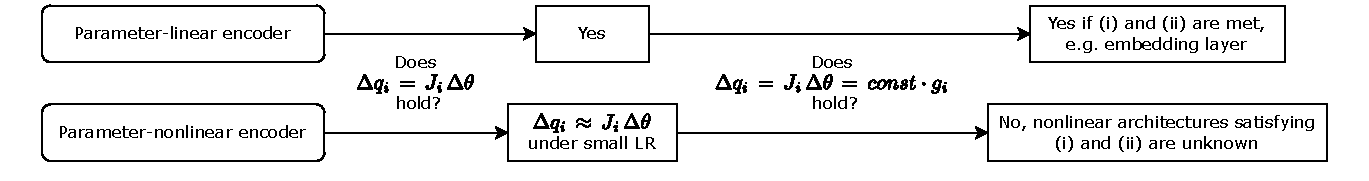
\includegraphics[width=\textwidth]{../draft_materials/figure_1_paper.pdf}
\caption{Mind map of Sections~2.1--2.4. Collinearity $\Delta q_i \parallel g_i$ holds only for a single embedding layer and a single linear layer (if the distinct inputs are pairwise orthogonal).}
\label{fig:sec2-mindmap}
\end{figure*}